
The aforementioned repository on GitHub is organized into separate folders for each class of the course, as shown in figure \ref{fig:github}.

\begin{figure}[!ht]
\centering
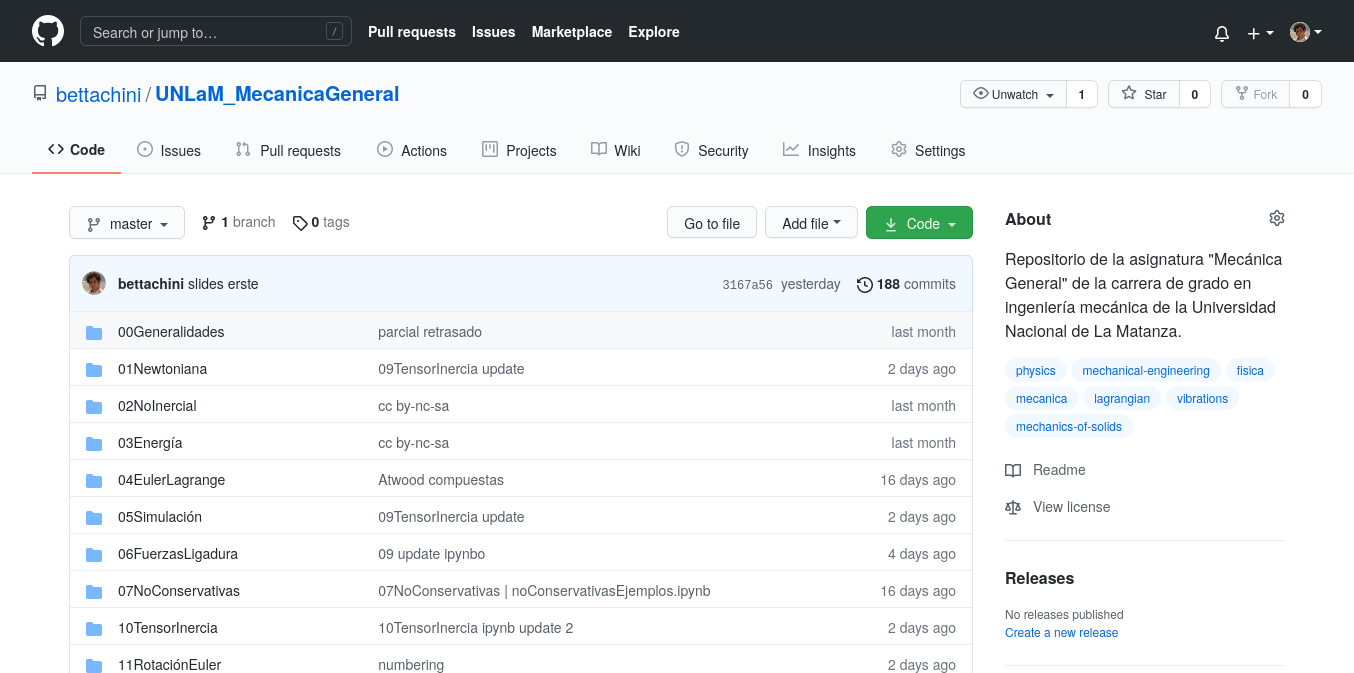
\includegraphics[width=\linewidth]{figuras/repositorioGithub.png}
\caption{Github repository: the students find the material organized in separate directories per class \cite{repositorio-victor}.}
\label{fig:github}
\end{figure}

There is a folder for each subject matter containing the Jupyter Notebooks for lessons and exercises as well as exercise set and occasional notes in the portable document format known by its acronym in English PDF.
This arrangement facilitates both the teacher and the students an overview of the material of each topic as well as verifying any updates to it.
In this way, the course material is publicly available to interested parties at \url{https://github.com/bettachini/MecanicaAnaliticaComputacional/} \cite{repositorio-victor} as long as they cite its origin and do not use it commercially as indicated by its Creative Commons CC-BY-NC-SA license \cite{creative}.
As the course is dictated in castillian (spanish) for the time being all material available in the repository is in that language.
